\section[For- and Background]{For- and Background}



\subsection{Certification Process}

\begin{frame}
  \frametitle{Getting Started}
  \begin{columns}
    \begin{column}{.5\textwidth}
       \centering
      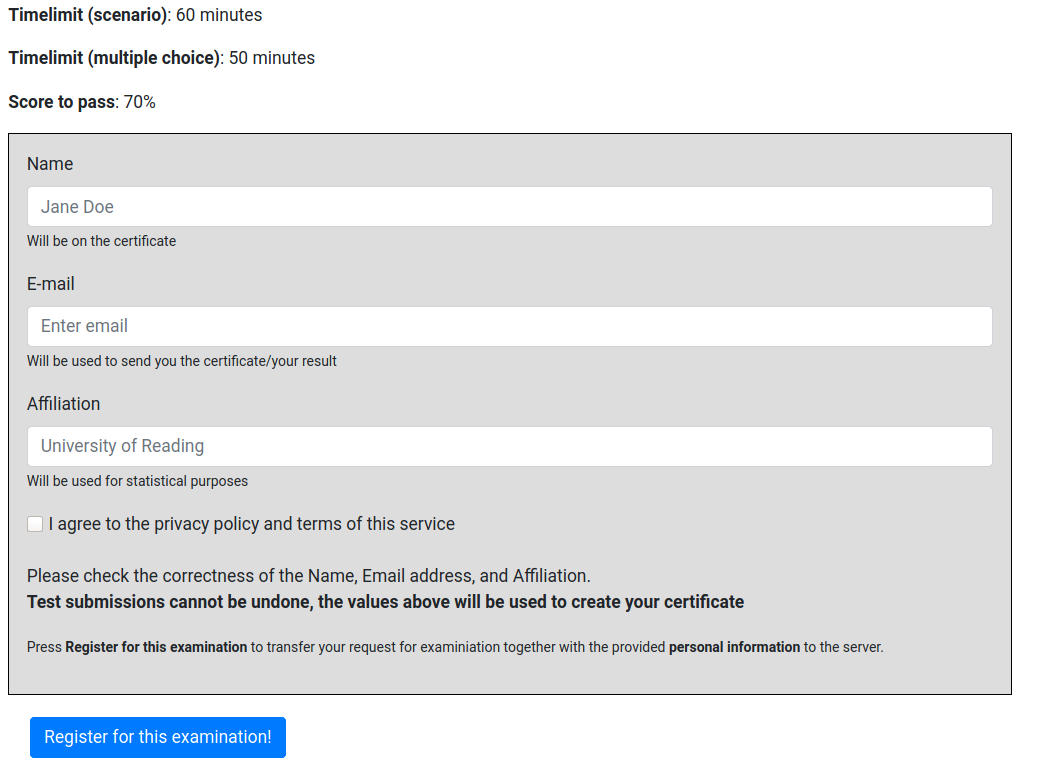
\includegraphics[width=0.9\textwidth]{images/getting_started}
    \end{column}
    \begin{column}{.5\textwidth}
      \begin{itemize}[<+->]
       \item navigate to the web page
       \item select the appropriate skill to be tested for
       \item submit Name (which will is needed for the certificate) \& and email
      \end{itemize}
      \pause
      $\curvearrowright$ a mail will be send containing links and keys for the actual exam (valid for 24 h)
    \end{column}
  \end{columns}
  
\end{frame}

\begin{frame}
 \frametitle{Background: Selecting the Questions}
 \begin{columns}
    \begin{column}{.5\textwidth}
       \centering
      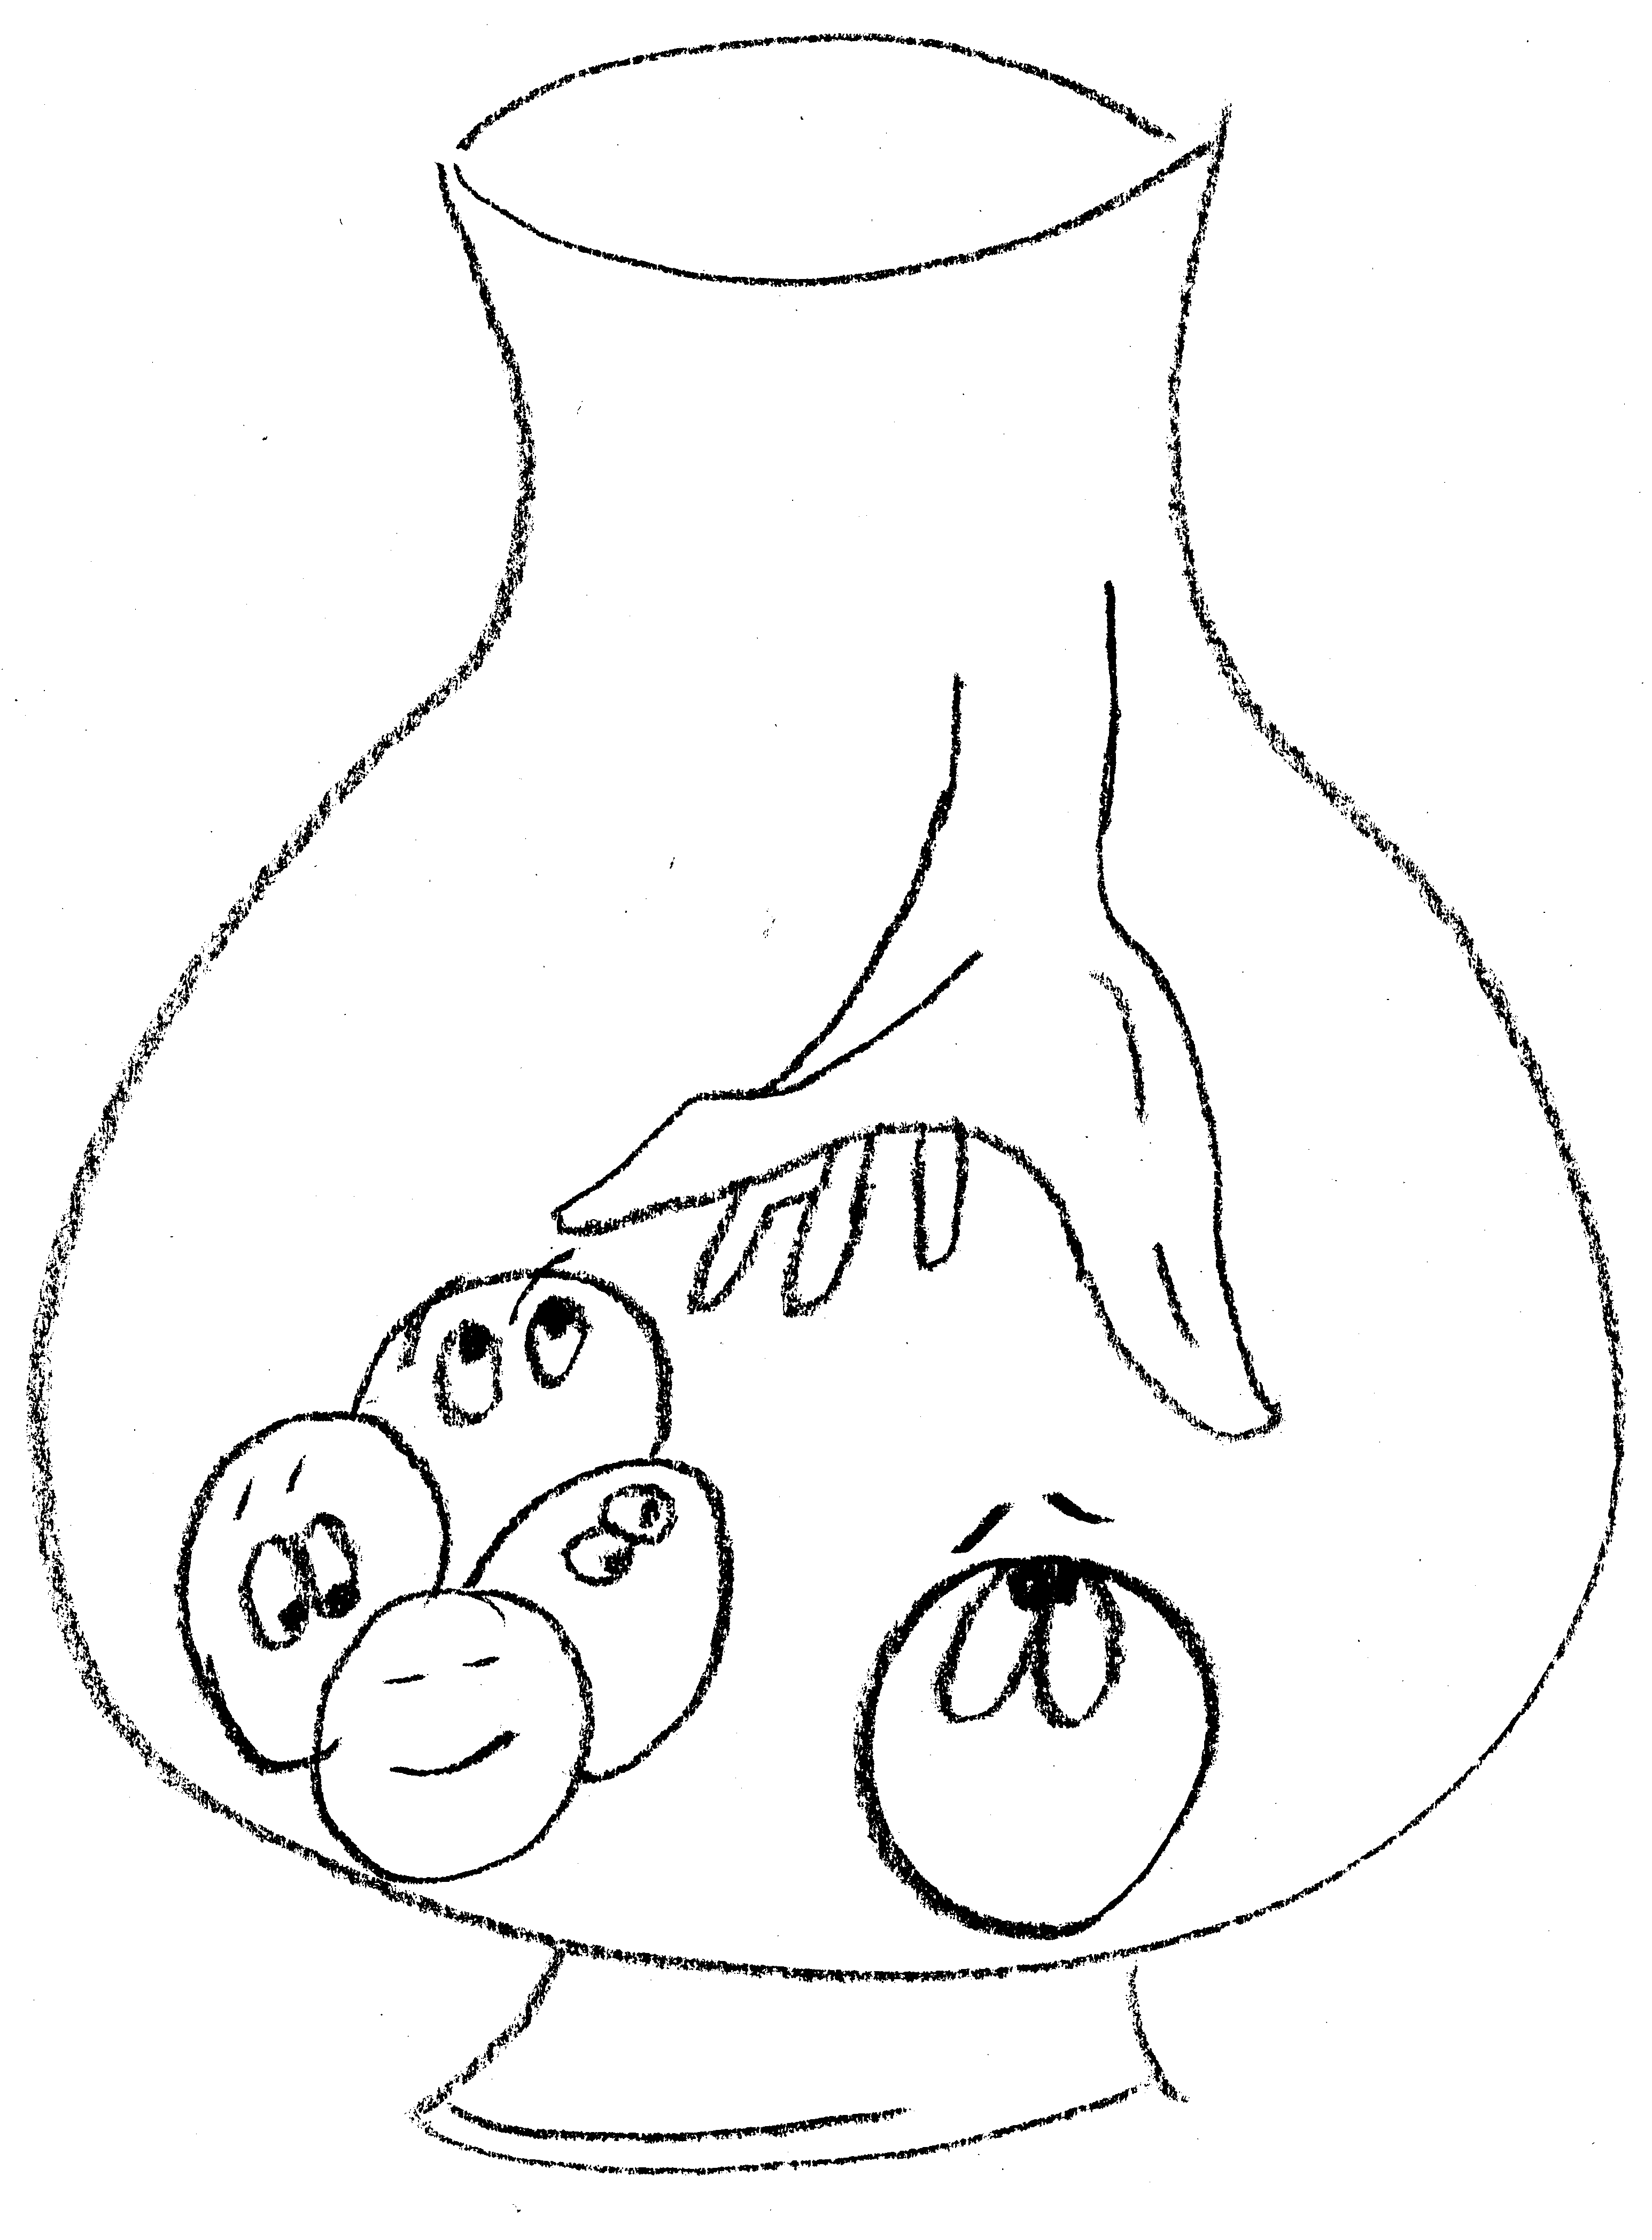
\includegraphics[width=0.6\textwidth]{images/urn}
    \end{column}
    \begin{column}{.5\textwidth}
      Questions are randomly choosen from a pool:
         the pool may itself be a bundle of sub-branches of the skill tree
              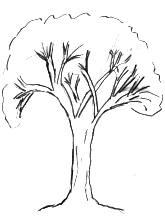
\includegraphics[width=0.1\textwidth]{images/tree_tiny}
        
      $\curvearrowright$ All examinations will be based on different sets of questions.
    \end{column}
  \end{columns}
\end{frame}

\begin{frame}
  \frametitle{On Cheating}
  \begin{columns}
   \begin{column}{.5\textwidth}
     \begin{enumerate}
      \item By confronting with random questions no perfect preperation can be accomplished.
      \item There is a time-limit per question.
      \item A registration prior to a test session is required.
     \end{enumerate}
    No online system without ID checks and other measures is safe against cheating! Yet, our measures will raise awareness.
   \end{column}
   \begin{column}{.5\textwidth}
       \centering
      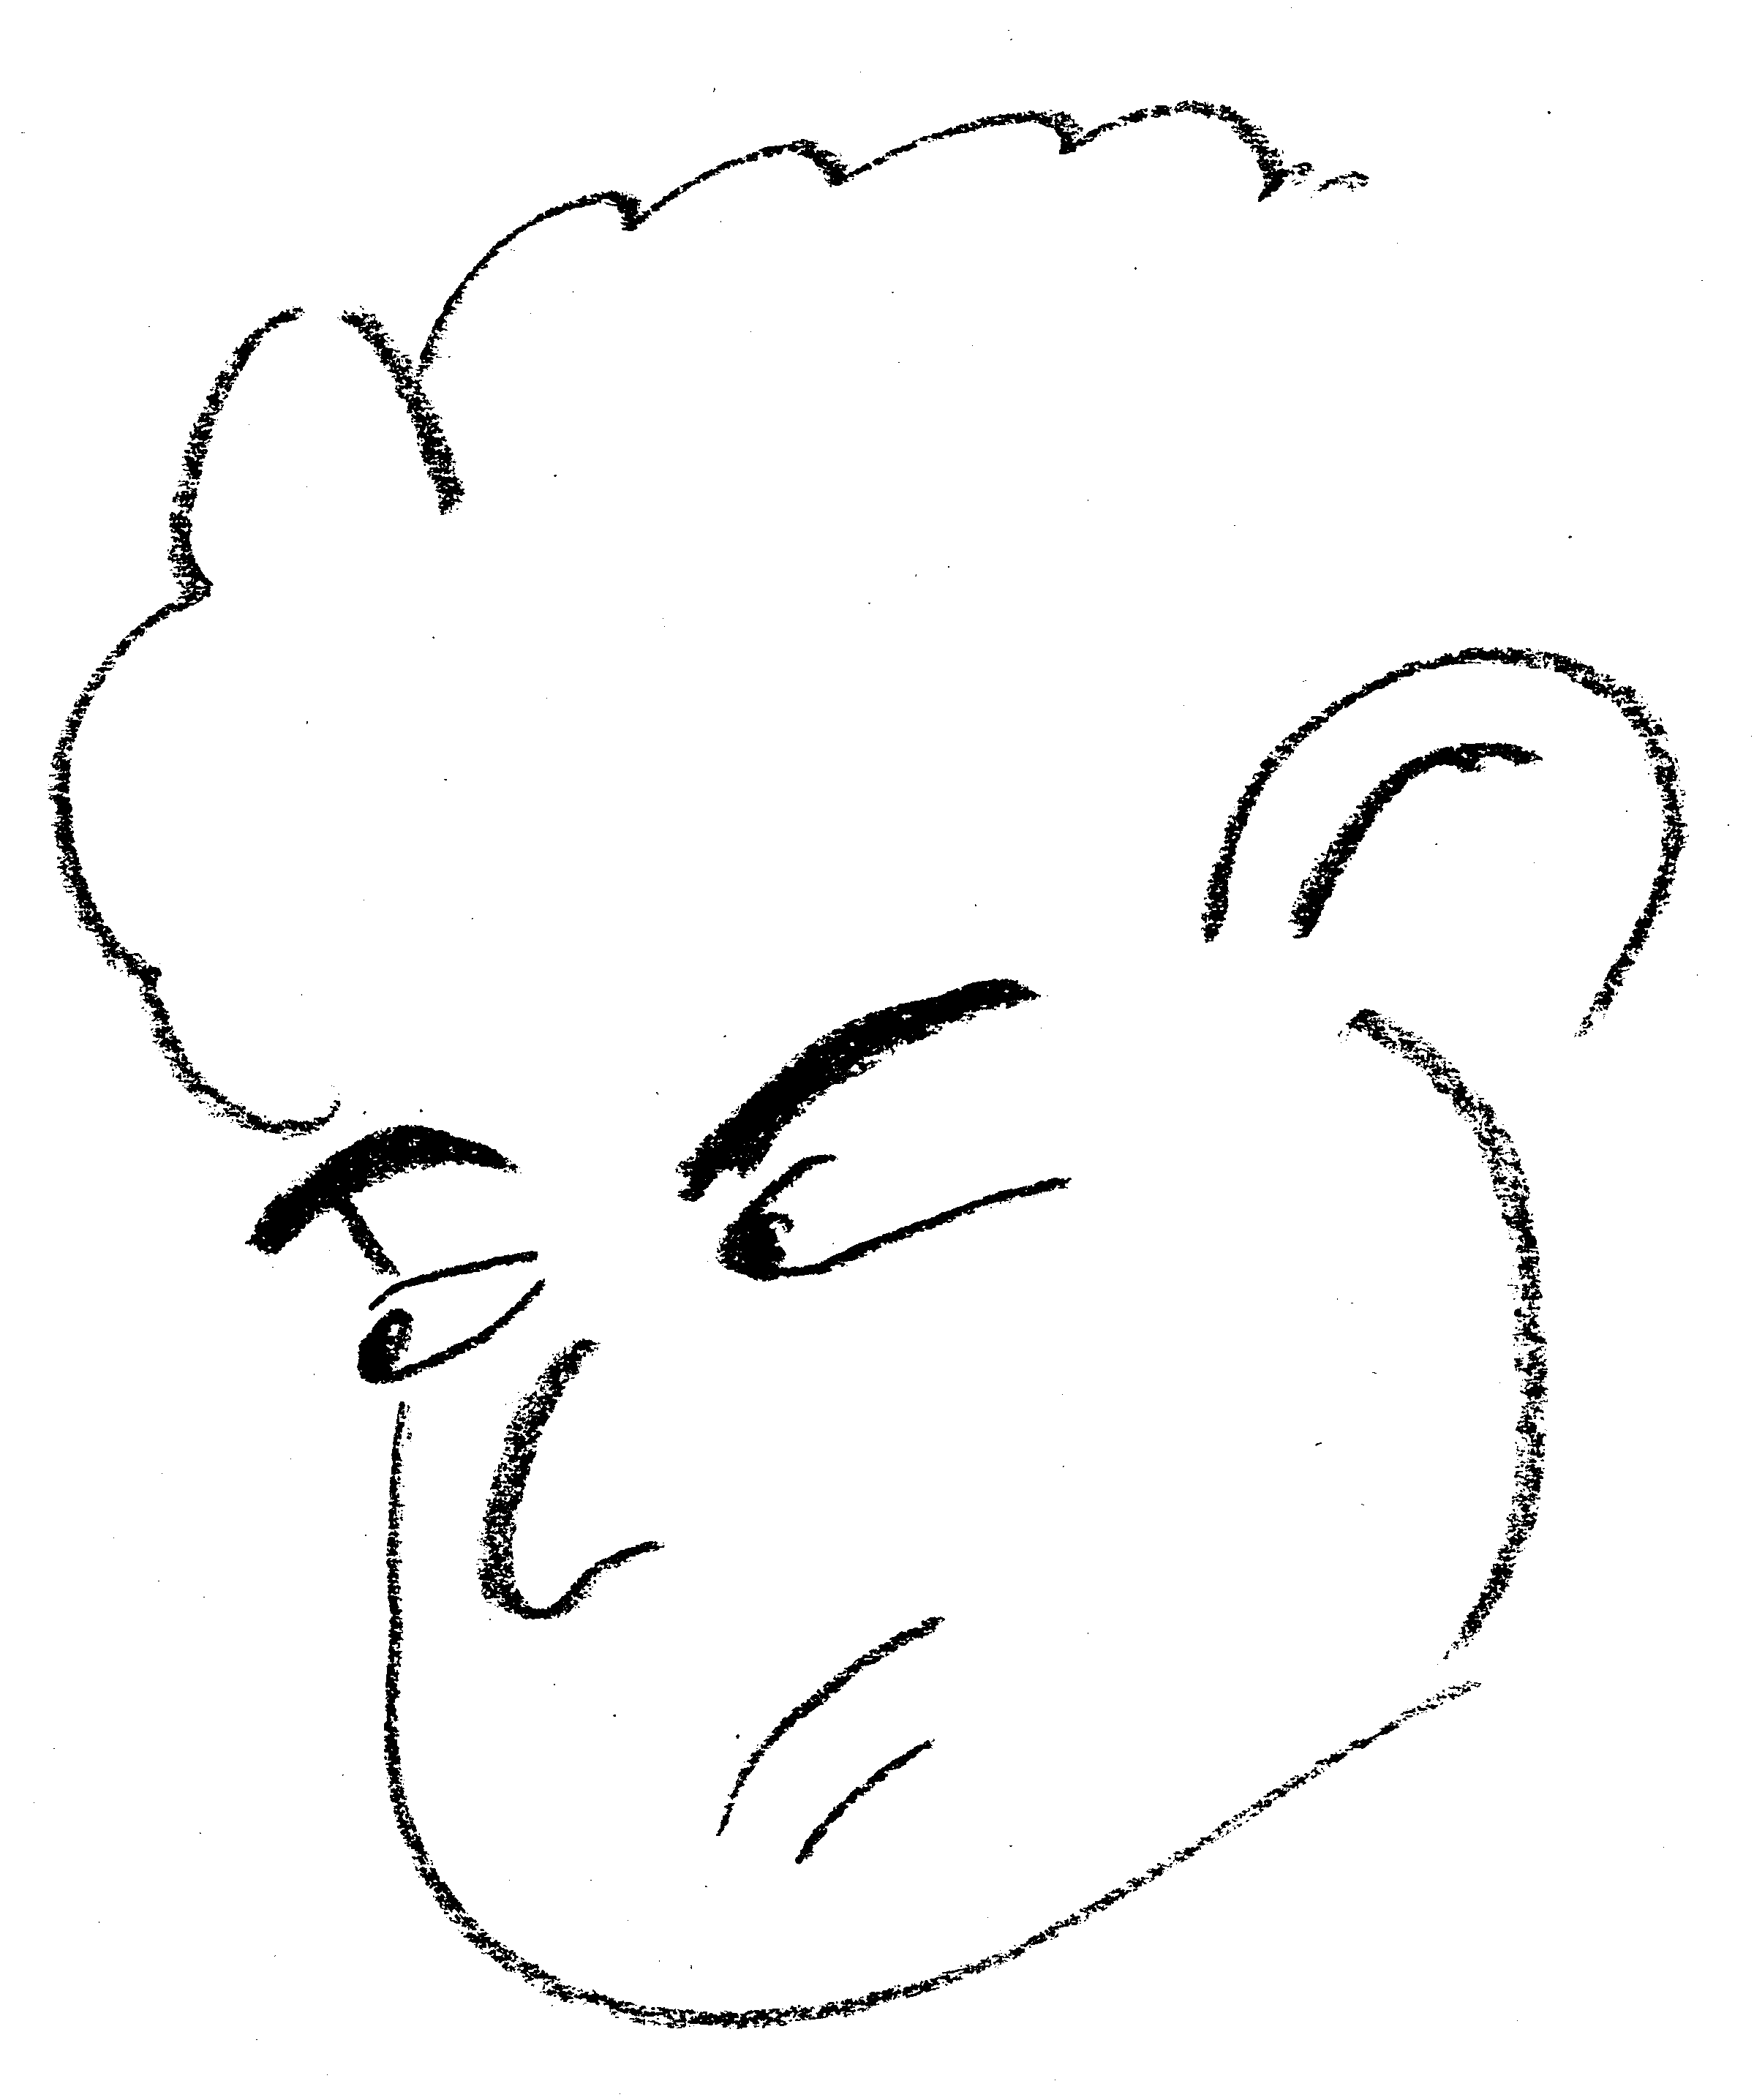
\includegraphics[width=0.6\textwidth]{images/cheating}
    \end{column}
  \end{columns}
\end{frame}

\begin{frame}
 \frametitle{Boosting Acceptance}
 \begin{columns}
   \begin{column}{.5\textwidth}
     Want to hire a scientist? \newline
     We intend to provide a (sub)set of question for prospective employers. This way they will have an idea of the background, if a solicitant waves a HPCCF-certificate.
   \end{column}
   \begin{column}{.5\textwidth}
       \centering
      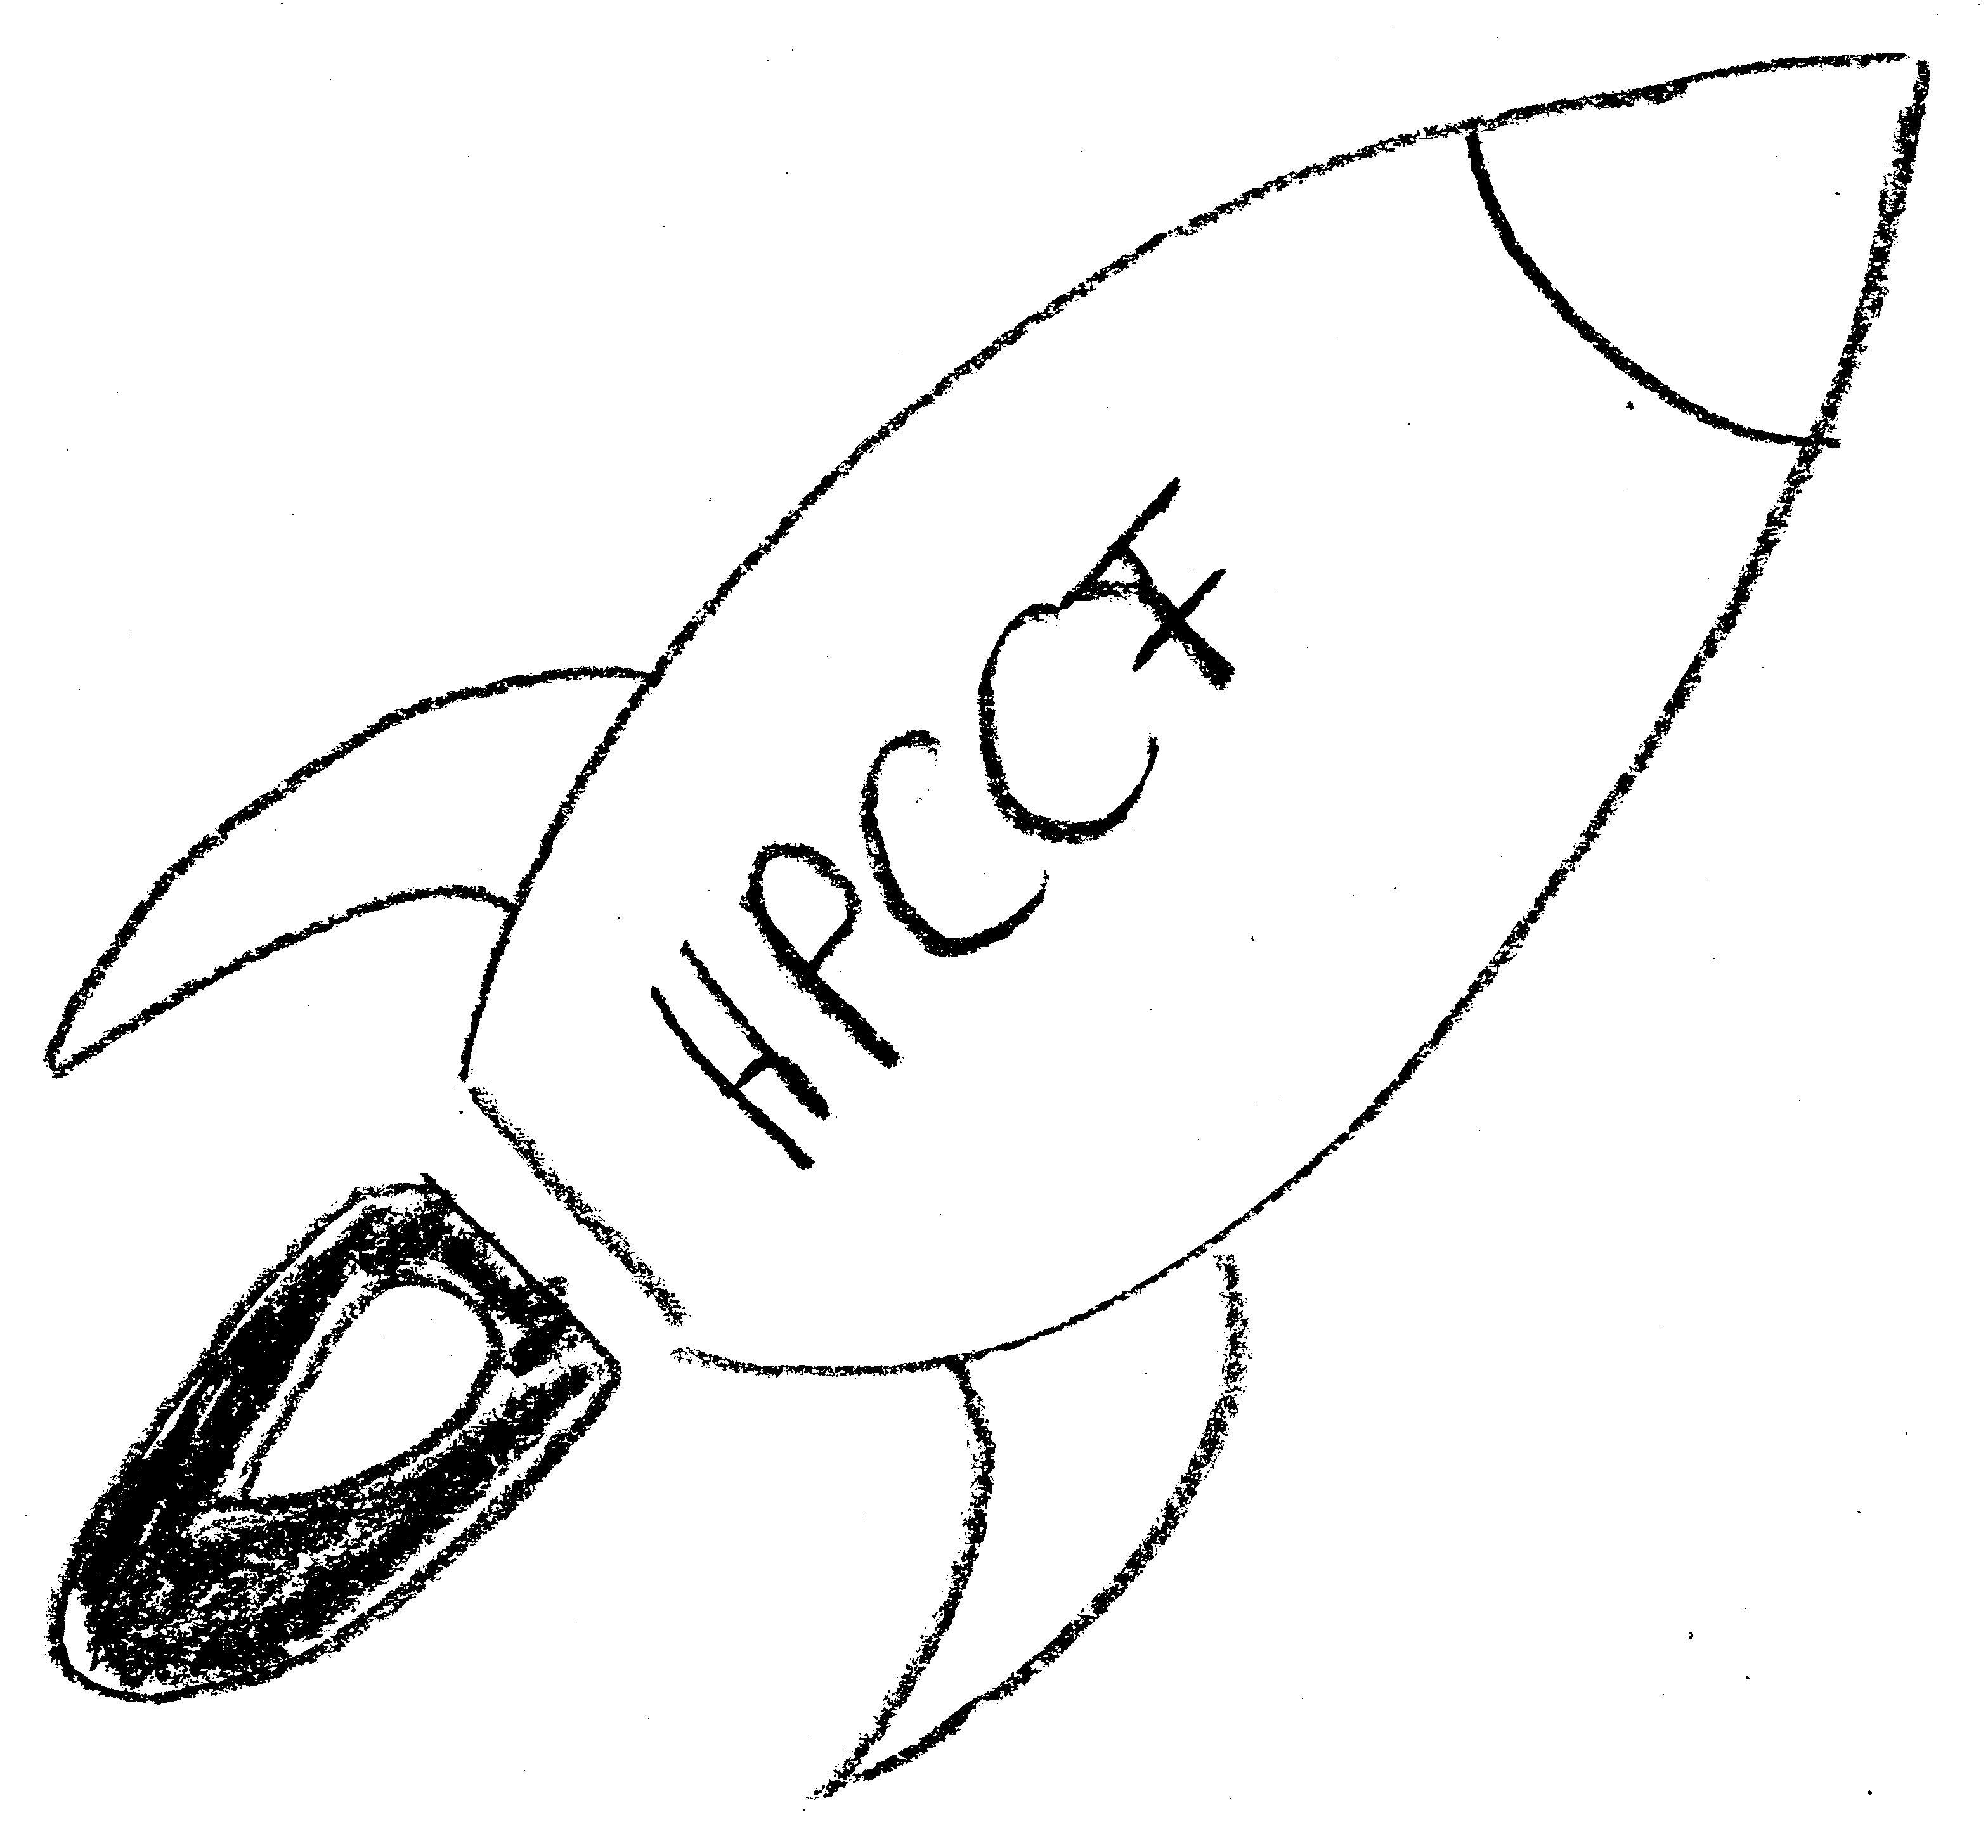
\includegraphics[width=0.6\textwidth]{images/hpccf_boost}
    \end{column}
  \end{columns}
\end{frame}

\begin{frame}
  \frametitle{Multiple Choice Questions}
  \begin{columns}
   \begin{column}{.5\textwidth}
      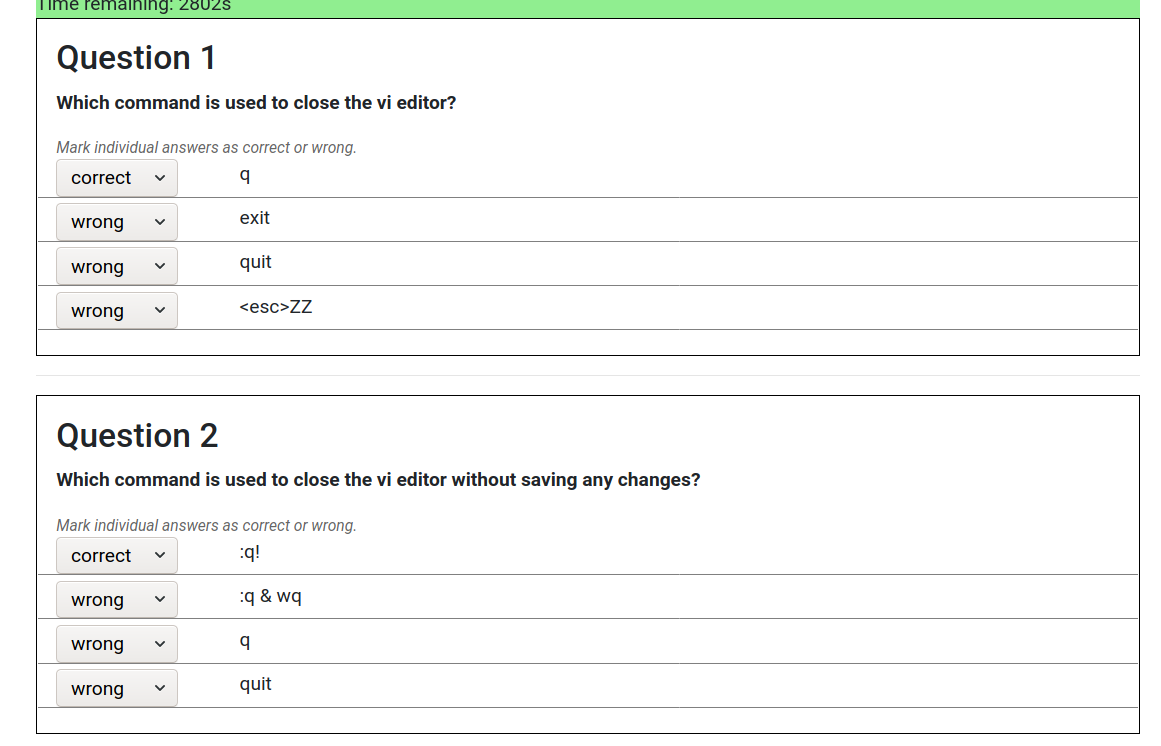
\includegraphics[width=0.9\textwidth]{images/questions_2}
   \end{column}
   \begin{column}{.5\textwidth}
       \centering
      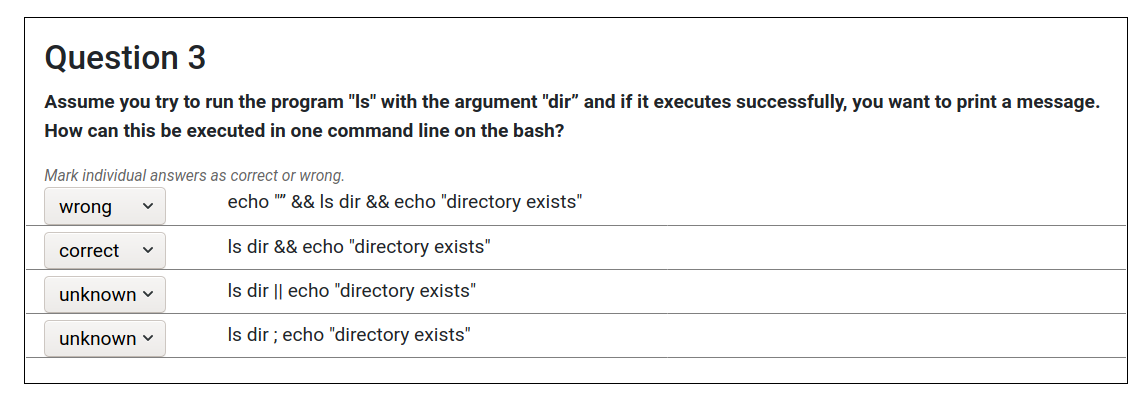
\includegraphics[width=0.9\textwidth]{images/question_1}
    \end{column}
  \end{columns}
\end{frame}

\begin{frame}
  \frametitle{Scenerio Based Questions}

\begin{tcolorbox}[colback=gray!5,colframe=green!40!black,title=Here:]
\footnotesize
In this task, you will need to run the program \texttt{terminator} and send a fixed sequence of signals to the program.
Note that this program is very sensitive to signals, very bad things may happen on the cluster if it is used incorrect. \textbf{Therefore, it is mandatory that you send the correct sequence of signals to the program and no other sequence.} 

We want to remind you that you can open multiple terminal sessions by opening the URL with the browser again.

Please send the following sequence of signals: 
\begin{enumerate}
  \item INT
  \item USR1
  \item 2
\end{enumerate}
\end{tcolorbox}

\end{frame}

\begin{frame}
  \frametitle{Scenerio Based Questions - Continued}
  \centering
  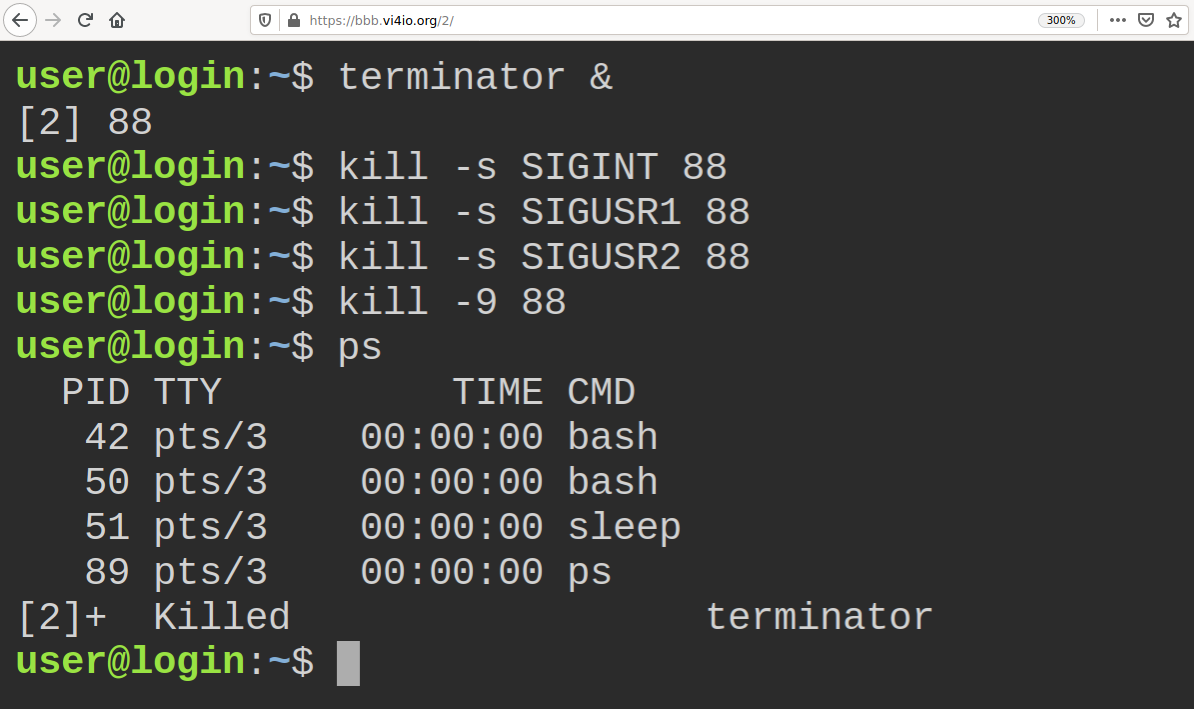
\includegraphics[width=0.65\textwidth]{szenario_3.png}

  Note: \texttt{SIGUSR2} != 2. Hence: Not full grade.
\end{frame}


% \begin{frame}
%   \frametitle{Improvements}
%   \begin{columns}[c, onlytextwidth]
%    \begin{column}{.4\textwidth}
%       \setlength{\partopsep}{0pt}
%       %\begin{minipage}{\textwidth}\vspace{0pt}
%        Bullet Point / Tick Boxes:\newline
%       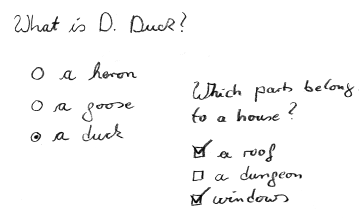
\includegraphics[width=0.9\textwidth]{mcq_ideal}
%       %\end{minipage}
% 
%       
%    \end{column}
%    \begin{column}{.55\textwidth}
%        \pause
%        \setlength{\partopsep}{0pt}
%       % \begin{minipage}{\textwidth}\vspace{0pt}
%         Syntax Highlighting:\newline
%       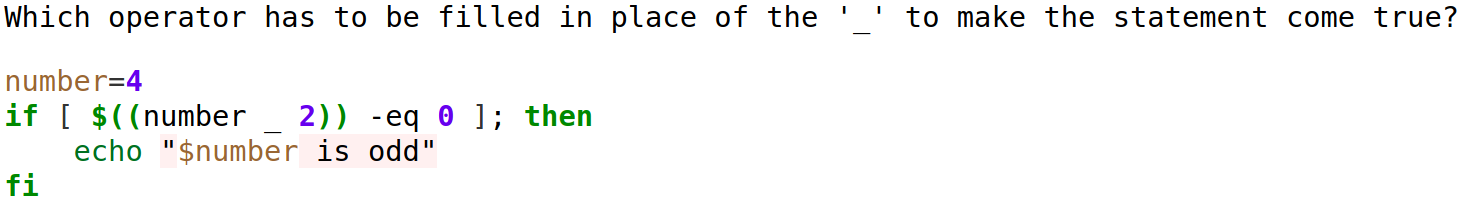
\includegraphics[width=0.9\textwidth]{syntax}\newline
%       \footnotesize{actual screenshot, not \LaTeX highlighting for the talk}
%        %\end{minipage}
% 
%       
%     \end{column}
%   \end{columns}
%   
% \end{frame}






